\section{Introduction}
Very Long Baseline Interferometry (VLBI) \cite{VLBIbook} is a type of
interferometry used in radio astronomy, in which data received at
several telescopes is combined to produce an image with very high
resolution. VLBI can be used for both astronomy and geodesy.  For
astronomy, VLBI provides high-resolution images of radio sources in
the sky, whereas in geodesy VLBI measures the location of the
telescopes and the Earth Orientation Parameters (EOP).

Astronomical research aims to study the sky and requires high angular
resolution. The resolution of the image increases linearly with the
size of the telescope dish. However, it is not possible to build
telescope dishes of arbitrary large size.  Instead, measurements of
several telescopes can be combined using VLBI to simulate a telescope
as large as the Earth. 
%By measuring the cross correlation of the signals between all
%telescope pairs, one is able to measure the angular Fourier components
%of the image in the sky.

\subsection{VLBI}
In order to approximate a telescope with a larger dish, multiple
telescopes can observe the same object, and the data can be combined
using interferometry. A pair of telescopes forms a baseline. The
maximal frequency is defined by the two telescopes farthest apart. Due
to the rotation of the earth, these projected distances change during
an experiment giving the possibility to measure a range of spatial
frequencies with a limited number of telescopes. The angular
resolution of the VLBI array depends on the maximum projected baseline
length, while the sensitivity depends on the number of telescopes and
the bandwidth. Because the radio emission has a broad white noise
spectrum it is most efficient to use two bit (4 level) sampling of the
signal. However the data rate is a limiting factor for the total
bandwidth, as Nyquist sampling is required.

In practice, the data is recorded at the telescopes on disk packs
during a VLBI experiment. After the experiment the disks are shipped
to a central institute, e.g. the Joint Institute for VLBI in Europe
(JIVE), for correlation. At JIVE, the data from the different
telescopes is played back and correlated by a dedicated hardware
correlator~\cite{EVNCorrelator}. The maximal capacity of this hardware
correlator is 16 telescopes at a data rate of 1Gbs each. There can be
several weeks between the experiment and the time when the correlated
data becomes available.

%\marginpar{NGHK: Check 16Mb/s in table}
\begin{table}
  \centering
  \begin{tabular}[c]{|l|l|l|l|l|l|}
    \hline
    Description & \# & \#  & data-rate & spect/prod & Tflops\\
    & telescopes & sub-bands & (Mb/s) &  & \\
    \hline
    \hline
    Fabric-demo &4 &2 &16 &32 &0.16\\
    1 Gb/s, full array  &16 &16 &1024 &16 &83.39\\
    future VLBI &32 &32 &4096 &256 &\verb|~|21457\\
    \hline
  \end{tabular}
  \caption{Network bandwidths and computing power needed for an {\it e}-VLBI
    experiment based on a XF architecture.}
  \label{tab:speed}
\end{table}
\subsection{{\it e}-VLBI}
In an electronic VLBI ({\it e}-VLBI) experiment \cite{szomoru-2004},
data from the telescopes is transferred directly over the internet to
JIVE, where it is streamed into the correlator in real time. The data
transport from the telescopes to JIVE goes over several networks like
local connections, paths provided by NRENs and the G\'EANT backbone in
Europe.

The sensitivity achievable using interferometry is proportional to the
square-root of the data rate and the number of telescopes, whereas the
angular resolution is proportional to the maximal distance between two
antennas. Hence, heavy requirements are put both on the network
connections and the computing power to achieve a good sensitivity, see
also Table~\ref{tab:speed}.

Transporting the data over the network has several advantages over a
traditional experiment. Obviously, the results of the experiments are
almost immediately available. This opens up the possibility to change
the course of an experiment based on earlier findings. Also, {\it
  e}-VLBI allows for real time analysis of the data and helps to
identify and resolve minor technical problems in the data collection
during the experiment.

Several experiments in the past have shown that real time {\it e}-VLBI
is possible. The EC funds the EXPReS project\footnote{EXPReS is made
  possible through the support of the European Commission (DG-INFSO),
  Sixth Framework Programme, Contract \#026642.}~\cite{EXPReS} which
aims at building a production-level {\it e}-VLBI instrument of upto 16
intercontinental telescopes connected in real-time to JIVE and
available to the general astronomy community.

\begin{figure}
  \centering
  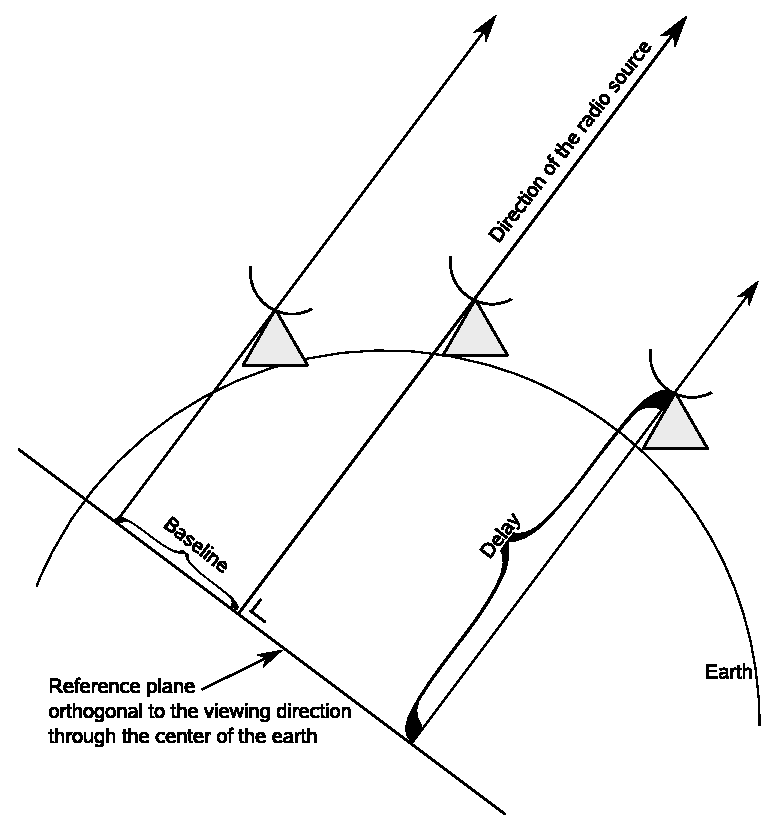
\includegraphics[width=.425\textwidth]
    {img/VLBI}
    \caption{Block diagram of the correlation.}
  \label{fig:correlation_diagram}
\end{figure}
\subsection{Correlation}
Correlation is the process by which data from multiple telescopes is
collected and combined to measure the spatial Fourier components of
the image of the sky. The high data rates and the optimizations
complicate the process.

Assume that we are correlating the signal of two telescopes. First,
both signals are delayed to account for the different time at which
the signal arrives at the telescopes, see
Figure~\ref{fig:correlation_diagram}. Next, a phase shift is performed
to compensate for the Doppler effect produced by the rotation of the
earth. This process requires very accurate timing information in the
data and a very detailed model of the geometry of the experiment. The
signals are now ready to be correlated.

During correlation, the first signal is delayed with discrete steps
and each delayed signal is multiplied with the second signal and then
integrated.  The output is a summation per delay step.

For more than two stations, each station is correlated with itself
(auto-correlation) and every other station (cross-correlation). Note
that the complexity is quadratic in the number of telescopes.

